\documentclass[11pt]{beamer}
\usetheme{Antibes}
\usepackage[utf8]{inputenc}
\usepackage{amsmath}
\usepackage{amsfonts}
\usepackage{amssymb}
\usepackage{graphicx}
\usepackage{multicol}

\author{Orosz Péter}
\title{Multiverzum Teória}
\setbeamercovered{transparent} 
\setbeamertemplate{navigation symbols}{} 
%\logo{} 
\institute{Miskolci Egyetem} 
%\date{} 
\subject{Bevezetés TEX-be} 

\AtBeginSection[]{
  \begin{frame}
  \vfill
  \centering
  \begin{beamercolorbox}[sep=8pt,center,shadow=true,rounded=true]{title}
    \usebeamerfont{title}\insertsectionhead\par%
  \end{beamercolorbox}
  \vfill
  \end{frame}
}

\begin{document}
	\begin{frame}
		\titlepage
	\end{frame}

	\begin{frame}
		\tableofcontents
	\end{frame}

	\section{Mi az a multiverzum?}
	\transdissolve
	\begin{frame}
		\begin{itemize}
			\item<1-> A multiverzum teória azt állítja hogy a mi univerzumunk csak egyike a megszámlálhatatlanul végtelen univerzumok közül.
			\item<2-> A Multiverzum a neve ezen univerzumok halmazának.
			\item<3-> Párhuzamos univerzumok, más univerzumok, alternív univerzumok és még sok már.
		\end{itemize}
	\end{frame}
	
	\section{Bizonyíték a multiverzumra}
	\transdissolve
	\begin{frame}
		\begin{multicols}{2}
			\begin{flushright}
				\Large \textbf{A LEGNAGYOBB BIZONYÍTÉKOK A MULTIVERZUM LÉTEZÉSÉRE}
			\end{flushright}
			\vfill\null
			\columnbreak
			\begin{itemize}
				\item<1-> \small A csillagok hosszú élettartama
				\item<2-> \small A szén(Carbon) bőséges mennyisége az univerzumunkban.
				\item<3-> \small A fotoszintézishez szükséges fény elérhetősége.
				\item<4-> \small A komplex sejtmagok stabilitása.
			\end{itemize}
		\end{multicols}
	\end{frame}
	
	\section{Fizikai bizonyíték}
	\transdissolve
	\begin{frame}
		\begin{multicols}{2}
			Ha egy szomszédos univerzum közelkerült a miénkhez és összeütközött azzal, akkor hátra kellet hagynia:
			\begin{itemize}
				\item Kozmikus mikrohullámú háttérsugárzást
				\item Galaxisok tuljadonságainak természetellenes megváltozása
			\end{itemize}
			\vfill\null
			\columnbreak
			\begin{figure}
				\centering
				\caption{Két univerzum ütközése}
				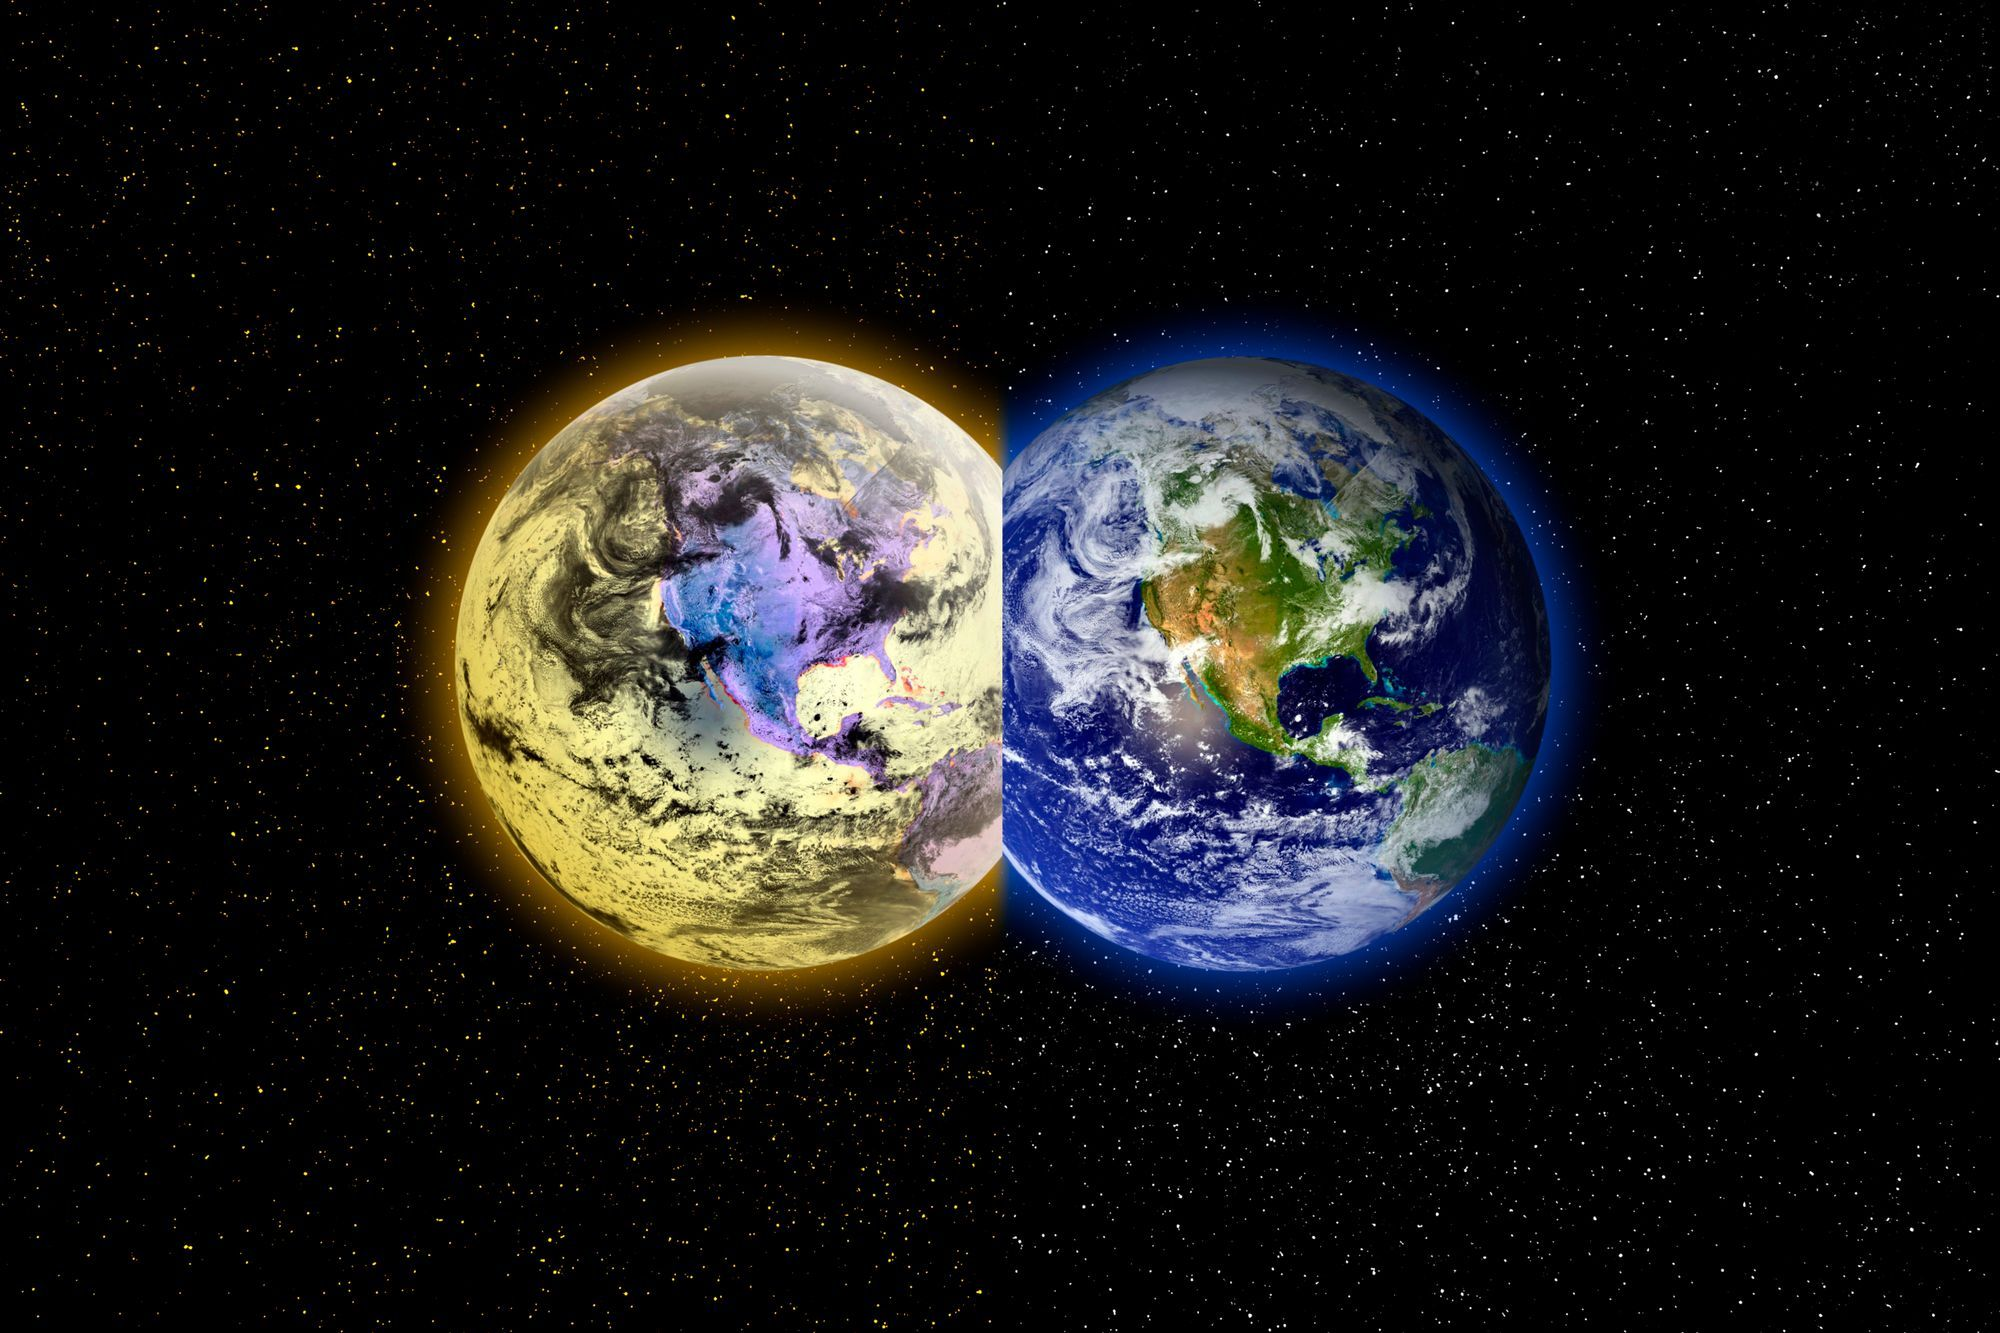
\includegraphics[scale=0.07]{utkozes.jpeg}
			\end{figure}
		\end{multicols}
	\end{frame}
	
	\section{Doppelgängers}
	\transdissolve
	\begin{frame}
		\begin{itemize}
		 \item<1-> Egy doppelgänger egy fizikailag teljesen megegyező személy valaki mással.
		 \item<2-> Régi időkben nagy balszerencsének az előjele volt ha valaki találkozott a doppelgänger-ével.
		 \item<3-> A multiverzum teória szerint a doppelgänger-ek a miénkből majdhogynem teljesen megegyező univerzumból kerültek át hozzánk valamilyen oknál fogva, de mivel univerzumaink annyira megegyező így a doppelgänger sem tudja hogy unverzumok között utazott.
		\end{itemize}
	\end{frame}
	
	\section{Multiverzum típusai}
	\transdissolve
	\begin{frame}
		\begin{enumerate}
			\only<1>{
			\item Buborék univerzumok
				\begin{itemize}
					\item Az "örök infláció" néven is ismert.
					\item Lényege, hogy a felfújódás a tér egyes szegleteiben megállt, míg máshol tovább folytatódott.
					\item Ennek következtében a megálló és felfújódó térrészek között "buborék univerzumok" létezhetnek.
					\item Ezekben az univerzumokban az alapvető fizikai állandók és a fizika törvényei teljesen eltérőek lehetnek.
				\end{itemize}
			}			
  			\setcounter{enumi}{1}
			\only<2>{
			\item Párhuzamos univerzumok
				\begin{itemize}
					\item A húrelméletből ered az az elképzelés, hogy az ismert és érzékelhető négy téridő dimenziónál több is létezhet, ahol más univerzumok a miénkhez hasonlóan négydimenziósak, de más dimenziókban léteznek.
					\item  Az elmélet egyik következtetése, hogy ezek a párhuzamos univerzumok fizikailag bár közel helyezkedhetnek el egymáshoz képest, de normál esetben nem érintkeznek egymással, azonban egyes elképzelések szerint az ősrobbanás oka két ilyen párhuzamos univerzum összeütközéséből eredeztethető, azaz ilyen esemény többször is megtörténhet.
				\end{itemize}
			}
  			\setcounter{enumi}{2}
			\only<3>{
			\item Elágazó univerzumok
				\begin{itemize}
					\item A kvantumfizika a világot valószínűségekkel írja le.
					\item Az elmélet lehetővé teszi, hogy minden lehetséges fizikai állapothoz meghatározható legyen egy valószínűség, amivel az adott esemény bekövetkezik, illetve megengedi azt is, hogy ezek mindegyike bekövetkezzen.
					\item Ekkor egy különálló univerzum jön létre, amiben az egyik esemény bekövetkezik, míg egy másik univerzumban egy másik esemény, és így tovább.
					\item Szemléletes példával egy útkereszteződéshez érve az egyik univerzumban a jobb oldali utat választjuk, míg egy másik univerzumban a bal oldali utat. 
				\end{itemize}							
			}
			\setcounter{enumi}{2}
			\only<4>{
			\item Matematikai univerzumok
				\begin{itemize}
					\item Egy elképzelés szerint a valóságot igazából a matematika nyelvén lehet leírni, és amit az érzékszerveinkkel érzékelünk, az ennek csak halvány, tökéletlen mása. Azonban matematikai struktúra sokféle létezhet, és mindegyik leírja a saját, független univerzumát. 
				\end{itemize}
			}
		\end{enumerate}
	\end{frame}
\end{document}
